\section{Software Structure}
The software structure is divided into ROS nodes, each with a specific functionality. 
Figure \ref{fig:software_structure} represents an abstract view of the message flow between the nodes. 
The following nodes are included:
\begin{itemize}
    \setlength{\itemsep}{1pt}
    \setlength{\parskip}{1pt}
    \setlength{\topsep}{1pt}
    \item \textbf{Camera Node}: This node is responsible for capturing RGB and depth images from the Realsense L515 camera and publishing them to the ROS network.
    \item \textbf{Detection Node}: This node subscribes to the RGB and depth topics, performs image segmentation, and publishes the results to the ROS network.
    \item \textbf{Mapping Node}: This node subscribes to the detection result topic and creates a 3D point cloud of the detected objects. It acts as an intermediate node between the detection and world nodes. It has information about the different reference frames and spins a thread to remove objects whenever they are removed from the environment.
    \item \textbf{World Node}: This node exposes the necessary services to interact with the world model.
\end{itemize}

\begin{figure}[H] % Use [H] to place the figure exactly here
    \centering
    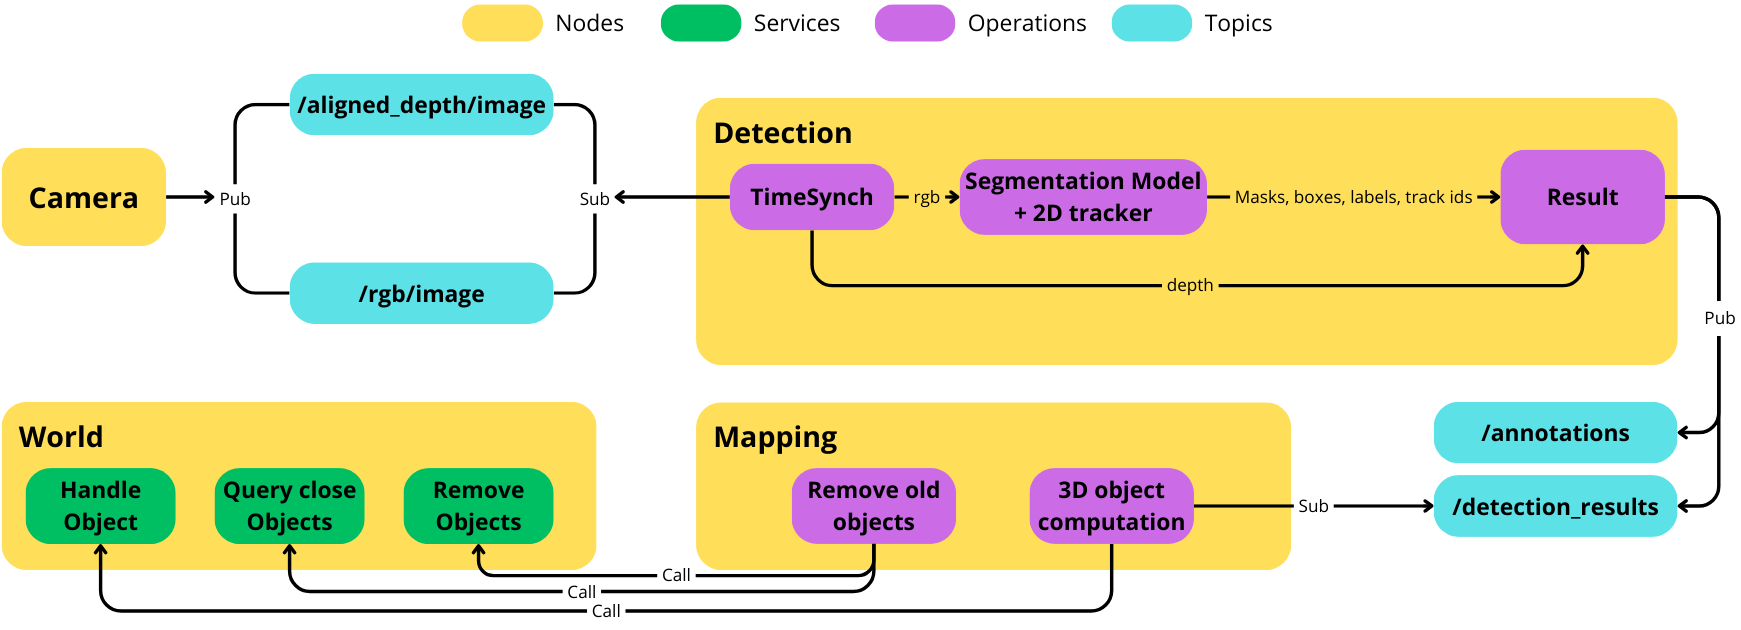
\includegraphics[width=1.0\textwidth]{figs/SW-struct.png}
    \caption{Software Structure}
    \label{fig:software_structure}
\end{figure}

\subsection[Detection Node]{Detection Node}
This node subscribes to the RGB and depth topics, performs instance segmentation, and publishes the results to the ROS network.
When RGB and depth images are published a callback function is triggered, this function acts a series of steps:
\subsubsection[YOLO]{YOLO - Instance Segmentation Model}
The YOLO model is used to perform instance segmentation, for further information about design choices and model details refer to section \ref{sec:instance_segmentation}.
This model has been implemented using the API provided by Ultralytics \cite{ultralytics_yolo_2023}.
In this application no batching is used since the model is running on a single image at a time.
This particular implementation offers also an implementation of the ByteTrack algorithm explained in section \ref{sec:byte_track} that allow to extract unique IDs for each detected object.

From this step we take only the segmentation masks, the unique IDs and the labels. 2D bounding boxes are not considered as 3D bounding boxes will be computed by from the objects point clouds.
\subsection[Mask Erosion]{Mask Erosion}
Since depth acquired from this particular camera tends to ...
